\section{Introduction}

Data collection processes proliferate due to the emergence of embedded
systems and sensor networks.  This provides opportunity to collect
large amounts of data. To be useful these data should be analysed and
processed by information systems. A typical processing, for instance,
is to detect eventual sensor failures or malfunctions and, if it is
possible, to reconstruct the faulty data. The acquired data instances
are bound to a timestamp, therefore correctness criteria must include
both data value and its timestamps. The sequences of data values
collected at specific timestamps are formalised as time series.

Time series are defined as a collection of observations made
chronologically.  In general, time series are acquired continuously
from a phenomena monitoring. The observations can be recorded at
regular intervals, such as hourly or daily, resulting in equi-time
spaced data; or at irregular intervals, such as recording when a pump
is open or closed, resulting in non equi-time spaced data. Time series
data are often voluminous \cite{fu11,keogh08:isax}, thus efficiently
storing and accessing them can be complex. Moreover, this is specially
critical when developing small embedded systems, whose resources
(capacity, energy or processing power) are constrained
\cite{yaogehrke02}.  Additionaly, non equi-time spaced data increases
the difficulty of processing.

Time series can be stored and managed by relational database
management systems that are usually queried using Structured Query
Language (\acro{SQL}) .
%
However, some authors
\cite{dreyer94,schmidt95,stonebraker09:scidb,zhang11} notice that the
use of \acro{SQL} system as a time series backend suffers from some
drawbacks.

\acro{NoSQL} or \acro{NewSQL} products are being developed in order to
increase the performance and flexibility of \acro{SQL} systems
\cite{atzeni13:relational_model_dead,stonebraker10,stonebraker09:scidb,zhang11}.
%
It is natural to consider them to store time series data. Even so, the
continuous acquisition nature of the time series poses an issue when
trying to store and analyse all the data \cite{keogh97}.

Compression techniques for time series are applied in two distinct
ways to face the challenges posed by time series data. First, to get
an approximation to the original signal in order to compute similarity
or pattern search analysis \cite{fu11,keogh01,last01}. Second, as a
compression and aggregation approach to store massive data streams
\cite{cormode08:pods,bonnet01}.
%
% Aixo no s'enten gaire que vol dir
Nonetheless, handling time series like data streams neither considers
adequately the time dimension nor computes the evolution of aggregated
parameters along time, which is interesting for monitoring purposes.

\emph{RRDtool} \cite{rrdtool} is a system that stores time series
aggregated in different resolutions. This allows to compact the data
and facilitates faster visualisations.
%
Even though, \emph{RRDtool} is a very specific application and
aggregation operations are limited to network monitoring.




\subsection{Contributions}

%TSMS

This paper introduces a model for a Data Base Management System
(\acro{DBMS}) that stores and manages time series data. These systems
are usually known as Time Series Data Base Management Systems
(\acro{TSMS}), \cite{dreyer94,last01}.
%
The introduced model organises the data in an aggregated way and it
allows to store time series using different time resolutions. This
characteristic is known as multiresolution. It is designed to satisfy
the requirements of bounded storage computers such as sensor systems.
%
Hence, our data model stands for a Multiresolution Time Series Data
Base Management System (\acro{MTSMS}).

The model is described in two steps. 
%
First, we introduce a \acro{TSMS} model that is devoted to time series
basic elements and operations.
%
Second, we introduce a \acro{MTSMS} model that adds multiresolution
capabilities to the first one. 
%
The model is mainly formalised using set algebra and, particularly,
relational algebra.  It also considers the time sampling
irregularities of time series. Moreover, it operates coherently with
the time dimension of time series.

In our model, multiresolution is the base for a lossy storage solution
that selects only the relevant data. This is close to multimedia
lossy compression methods where meaningless data is discarded in
favour of size.

Multiresolution requires to aggregate several data instances into a
single one. This requires an aggregation function that is tied to the
specific semantics of the actual data. Because of this, aggregation
functions are set as an independent object of the main model.  Users
can define new aggregation methods which are better suited for
specific fields.

The model also introduces the concept of time series representation
function.  This allows users to define different operators considering
the behaviour of time series in different contexts. This is important
to manage the specific semantics of the stored time series. For
instance, \emph{RRDtool}-like specific counter time series
aggregations would be defined based on this facility. Furthermore,
representation functions are formalised as an independent object of
the main model.



\subsection{Outline}

This manuscript is organised as
follows. Section~\ref{sec:related-work} introduces previous work that
concerns \acro{TSMS} and \acro{MTSMS}.  The motivation for
multiresolution is shown in Section~\ref{sec:features}.  The
\acro{TSMS} model is explained in Section~\ref{sec:model:TSMS} and the
\acro{MTSMS} model is explained in Section~\ref{sec:MTSMS}.  In
Section~\ref{sec:implementation} we describe an implementation of the
\acro{TSMS}+\acro{MTSMS} model.  Section~\ref{sec:example} is devoted
to a real data multiresolution database example.  Finally,
Section~\ref{sec:concl-future-work} offers some conclusions.




\section{Previous work}
\label{sec:related-work}

In this section, we describe some previous work related to time series
storage. It is described in three parts: first we introduce some known
database management systems approaches for time series, second we
explain how compression techniques are applied to leverage time series
storage, and last we review time series storage systems based on the
data streams paradigm.

\todo{CHANGE: s'hauria d'afegir el següent comentari}

% 1. Constatar que no n'hi ha de semblants 

%2. Que notem com altres treballs intenten resoldre els problemes de sèries temorals

% 3. Aclarir que hi ha temes parallels que ens serveixen dinspiracio

% Alguna cosa així?:
The formalism of multiresolution is novel. However, some of the
multiresotion features can also be find in other works.  Especially,
some other approaches when treating time series must be noted as they
could be used in the multiresolution model. 


\subsection{Database approaches}

According to some authors, \acro{TSMS} should be considered as a
specialized relational \acro{DBMS}~\cite{last01}.  Segev and
Shoshani~\cite{segev87:sigmod} propose a structured language for
querying \acro{TSMS}. Their time series structures include the notion
of regularity and temporal representation and their operations are
\acro{SQL}-like.  Dreyer et al.~\cite{dreyer94} suggest the
requirements of a special purpose \acro{TSMS} and base the model on
five basic structural elements: events, time series, groups, metadata
and time series bases. They implement a \acro{TSMS} named
\emph{Calanda} which includes calendar operations, it allows grouping
of time series and it operates with simple queries. They exemplify it
with financial data. In~\cite{schmidt95} \emph{Calanda} is compared
with temporal systems designed for time series.
 
Other authors consider array database systems well suited to
\acro{TSMS}.  \emph{SciDB}~\cite{stonebraker09:scidb} and
\emph{SciQL}~\cite{zhang11} are array database systems intended for
science applications, in which time series play a principal role. They
structure time series into arrays to achieve multidimensional analysis
and they store other data into tables.  \emph{SciDB} is based on
arrays which, according to the authors, allow to represent time
series.  In contrast, \emph{SciQL} defines time series as a mixture of
array, set, and sequence properties and exhibits some time series
managing characteristics that include time series regularities,
interpolation or correlation queries.
% However,
% difference between tables and arrays seems too physical and leads to
% ambiguity when representing time series.  
% Our TSMS model proposes time
% series as firmly based on relational algebra, clarifying this
% ambiguity and describing them coherently in terms of information
% systems theory.


Bitemporal \acro{DBMS}, sometimes referred directly as temporal data,
is a database field that inherently considers temporal dimension of
data. Bitemporal data manages historical data and events in databases
by associating pairs of \emph{valid} and \emph{transaction} time
intervals to data.  Bitemporal data and time series data are not
exactly the same and so cannot be treated
interchangeably~\cite{schmidt95}, however, there are some similarities
that can be considered. Moreover, \acro{DBMS} research represents
bitemporal data as relations extended with time intervals attributes
and extends relational operations in order to deal with related time
aspects~\cite{jensen99:temporaldata,date02:_tempor_data_relat_model}.
In this paper, we formalise time series in a similar way as how
bitemporal data is formalised for relational \acro{DBMS}.
% On the other hand, some bitemporal time concepts might be taken
% into account by \acro{TSMS}, such as the discussions about time
% granularities.



\subsection{Compression approaches}

% As \acro{TSMS} suffer from problematic properties of time
% series, like the ones we describe in
% Section~\ref{sec:model:properties} mainly the huge data volume,
% compression techniques are used.  Next, we summarise some current work
% in \acro{TSMS} with compression.

Oetiker's \emph{RRDtool}~\cite{rrdtool,lisa98:oetiker} is a free
software database management system. It is designed to be used for
monitoring systems. Because of this, it is focused to a particular
kind of data, gauges and counters, and it lacks general time series
operations. \emph{RRDtool} can store multiple time resolution data,
however Plonka et al.~\cite{lisa07:plonka} evaluated \emph{RRDtool}
performance and found limitations when storing a huge number of
different time series. They suggest a caching system on top of
\emph{RRDtool} as a solution.
%
Weigel et al.~\cite{weigel10} advocate a similar approach named
\emph{TSDS} that caches queries by aggregate parameters.  In his
paper, the authors state that other systems only show subsets of data
but it is also necessary to show data in their complete time span.
They develop the software package \emph{TSDS} where time series are
fully stored and then queried by date ranges or by applying different
filters and operations to the time series data.  
%
% No se si ajuntar en un paragraf al final de l'apartat
%
Our \acro{MTSMS} model is a generic approach to the multiresolution
inspired on \emph{RRDtool}. We define it open so that users can define
any attribute aggregate functions.


Deri et al.~\cite{deri12:tsdb_compressed_database} suggest
\emph{Tsdb}, a lossless compression storage \acro{TSMS} for time
series that share the same time instants of acquisition. Different
time series are stored grouped by the time of acquisition instead of
in a isolated way.  They compare \emph{Tsdb} with \emph{RRDtool} and
with a relational product. As a consequence of \emph{Tsdb} structure,
they achieve a better measure addition time but a worse global
retrieval time as data have to be contiguously regrouped. However,
when the measurements have same time this is seen as the same time
series in a \acro{MTSMS}, so it would be interesting to use this
implementation architecture of shared time arrays in \acro{MTSMS} for
resolution subseries with same delta time in order to achieve better
performance requirements when having much equal acquired time series.


Some lossy compression techniques for time series are devoted to the
optimal approximation representation. They seek to balance between the
least data that can reconstruct the original signal and the least
error. Keogh et al.~\cite{keogh01} cite some possible approximation
representations for time series such as Fourier transforms, wavelets,
symbolic mappings or piecewise linear representation. They remark this
last one as very usual due to its simplicity and develop a system
called \emph{iSAX}~\cite{keogh08:isax,keogh10:isax} in order to
analyse and index massive collections of time series. They describe
that the main problem is in the indexing of time series and they
propose methods for processing efficiently. The first method proposed
is based on a constant piecewise approximation. The time series
representation obtained with \emph{iSAX} allows reducing the stored
space and indexing faster with the same quality as other more complex
representation methods.  These compression techniques are candidates
for being used as attribute aggregate functions in the \acro{MTSMS}
model, as instance it would be interesting to define aggregations in
the frequency domain of time series.


 


\subsection{Data stream approaches}

\emph{Cougar}~\cite{bonnet01} is a sensor database system that has two
main structures: one for sensor properties that are stored into
relational tables and another for time series coming from sensors that
are stored into data sequences. Time series have specific operations
and can combine relations and sequences. \emph{Cougar} target field is
sensor networks, where data are stored distributed in different
locations. Queries are resolved combining sensor data in a data stream
abstraction that improves processing performance.

Time series as data streams are also considered when statistically
aggregating data in order to do fast approximate queries with
compressed data. Cormode et al.~\cite{cormode08:pods} develop
aggregation techniques that allow to give more weight to recent
data.  
%
% Veure on colocar
%
Our \acro{MTSMS} model applies a similar approach to time series. It
allows to weight more recent data over older one. Additionally it
copes well with multiple aggregations and time irregularities.
%
Dou et al.~\cite{dou14:historic_queries_flash_storage} create index
structures as multiresolution aggregates, like average, count, or top,
for historical data managed in flash storage. They consider a specific
storage solution based on a register with pointers similar to the
multiresolution storage in \emph{RRDtool}~\cite{lisa98:oetiker}.






\section{Multiresolution motivation}
\label{sec:features}

A \acro{TSMS} is a special purpose \acro{DBMS} devoted to store and
manage time series.  The main objective of \acro{TSMS} is to gather
two areas of study: time series analysis and \acro{DBMS}.  Time series
analysis formalises a great amount of algorithms and methodologies
that apply to time series, with a main focus on improving
efficiency. \acro{DBMS} theory formalises systems that store and
operate with data, currently the relational model is the referent
\cite{date:introduction}.



In time series analysis there are some common generic operations.
Most of these operations deal with the time given the nature of data.
Usual operations include querying time intervals, finding time
correlations, or calculating distances between two time series. In
all these operations \acro{TSMS} must consider the temporal coherence
of the time series.  In the context of statistics, aggregation of time
series is also a common operation. Aggregate means to summarise a time
series subset by a smaller set of measures. Statistic indicators like
the mean, the maximum, or the mode, for instance, summarise time
series into one only measure.

In the discrete context, a time series is defined as a set of value
and time pairs. Furthermore, a time series has a continuous nature as
it comes from a phenomena evolution along time. As a result,
\acro{TSMS} operations may deal with this time series nature by
methods of interpolation or approximation.


A \acro{MTSMS} proposes a \acro{TSMS} with multiresolution
capabilities.  A \acro{MTSMS} schema represents a time series using a
set of different resolutions.  The multiresolution concept comes from
thoroughly analysis of \emph{RRDtool} \cite{rrdtool}.  Our objective
is to formalise the main features into an abstract model and to
incorporate adequate generality in order to describe \acro{MTSMS} as
fully as a \acro{TSMS}.



As a summary, \acro{MTSMS} improve \acro{TSMS} features in various aspects:
\begin{itemize}

\item Voluminous data. Monitoring systems capture a huge amount of
  data from sensors. In order to be able to process these data,
  their volume must be reduced. One of the features of the
  multiresolution approach is to select and store only the most
  interesting segments of data. This segments are seen as different
  resolutions for the same time series and the user can configure how
  they are extracted and summarised by defining different time steps
  and functions. Multiresolution can also be useful when graphing time
  series allowing the user to select the best time range and time
  step that fits into the screen; there is no need to process with
  more quantity of data than the one that can be
  shown.

\item Data validation. Monitoring systems capture data but can cause
  some drawbacks that will affect later the process of time series
  analysis. Main problems are found when monitors can not capture
  data, known as gaps, or capture data erroneously, such as outlayers
  \cite{quevedo10}.  The multiresolution attribute functions is
  designed to cope well with validating, filtering and reconstructing
  with these unknown data in order to keep a consistent
  history.

\item Data time regularising. Another monitoring side effect happens
  when the sampling rate is not constant, that is when the resulting
  data are not equi-time spaced. This irregularities can come from
  sampling jitters in periodic sampling or from non-periodic
  event-based sampling \cite{kopetz11:realtime}. One multiresolution
  consolidation objective is to regularise the time interval when
  processing a time series, therefore each resulting time series
  segment has a regular time resolution. Besides obtaining regular
  time series, this feature can also be used in order to consult other
  resolutions from a time series, such as changing a daily acquired
  time series to a yearly step summary.


\item Data summaries. Time series analysis typically focuses on
  reconstructing the original signal. However, the user objective in a
  database system is to consult some information. The multiresolution
  approach allows a lossy compression storage solution for data. Therefore
  it can be regarded as to extracting the interesting data and
  then storing them. The selected data must be determined a
  priori assuming the context where the future queries will be done.
\end{itemize}


However sometimes it may also be useful to complement \acro{MTSMS}
with other \acro{DBMS}. Not only to store the original values as a
long-term deposit consulted offline, but also to store time series'
metadata such as units of values, sensor localisation, classification
tags, last measured value, etc.



\subsection{Motivation example}

Figure~\ref{fig:mtsms:sequence} shows an example of a multiresolution
summary for a time series.  It shows a snapshot in time spanning from
time 0 to 9 and supposing that the temporal point `now' is between 9
and 10. At the top of the figure there is a plot of a time series with
time axis in general units of time (u.t.) and with value axis in
undetermined units. The `now' point shows when the snapshot has been
taken, so the time before is the past and the time after is the
future, whose elements are plotted in discontinuous marks. The
\emph{init} point shows when the database system has started sampling,
so data in time before are unknown; the starting point is indicated as
zero u.t.\ and the previous unknown time points have negative units.


\begin{figure}
  \centering
  %\tikzsetnextfilename{fig_mtsms_sequence}
  %%\usetikzlibrary{positioning}
\begin{tikzpicture}[scale=0.77, every node/.style={transform shape}]

  %referencia
  \node (-6) {};

  \foreach \x in {-5,...,12}
  {
    \pgfkeys{/pgf/number format/.cd,int trunc}
    \pgfmathparse{abs(\x)}
    \let\absx=\pgfmathresult
    \pgfmathparse{\x-1}
    \let\antx=\pgfmathresult
    %time
    \node[node distance=1mm] (\x) [right=of \antx] 
    {\ifnum\x<11 \x \else \phantom{9} \fi};

    %graph values
    \node [above=\absx mm of \x] 
    {\ifnum\x=10 \color{gray} \fi \ifnum\x<11 $\bullet$ \fi};    

    %values
    % \node[rectangle,draw] (s\x) [below=of \x] 
    % {\ifnum\x<10 \pgfmathprintnumber{\absx} \else \phantom{9} \fi};
    \ifnum\x<10
    \node[rectangle,draw] (s\x) [below=of \x] 
    {\pgfmathprintnumber{\absx}};
    \else
    \node[rectangle,dotted,draw] (s\x) [below=of \x] 
    {\phantom{9}};
    \fi
  }

  \node [below=of 10] {\color{gray}10}; 
  

  
  %rd: 5s |inf| mean
  \node [circle,draw] (rd5-5) [below=3cm of s-5] {u};
  \node [circle,draw] (rd50) [below=3cm of s0] {u};
  \node [circle,draw] (rd55) [below=3cm of s5] {3};
  \node [circle,dotted,draw] (rd510) [below=3cm of s10] {\color{gray}u};
  \node [below=3.3cm of s10] {\color{gray}8};
 
  \draw[->,bend right] (s5) to (rd55);
  \draw[->,bend right] (s4) to (rd55);
  \draw[->,bend right] (s3) to (rd55);
  \draw[->,bend right] (s2) to (rd55);
  \draw[->,bend right] (s1) to (rd55);

  \draw[->,dotted,bend right] (s10) to (rd510);
  \draw[->,bend right] (s9) to (rd510);
  \draw[->,bend right] (s8) to (rd510);
  \draw[->,bend right] (s7) to (rd510);
  \draw[->,bend right] (s6) to (rd510);

  
  %rd: 3s |inf| mean
  \node [circle,draw] (rd3-3) [below=of s-3] {u};
  \node [circle,draw] (rd30) [below=of s0] {u};
  \node [circle,draw,fill=white] (rd33) [below=of s3] {2};
  \node [circle,draw,fill=white] (rd36) [below=of s6] {5};
  \node [circle,draw,fill=white] (rd39) [below=of s9] {8};
  \node [circle,dotted,draw] (rd312) [below=of s12] {\color{gray}u};

  \draw[->] (s3) to (rd33);
  \draw[->] (s2) to (rd33);
  \draw[->] (s1) to (rd33);

  \draw[->] (s6) to (rd36);
  \draw[->] (s5) to (rd36);
  \draw[->] (s4) to (rd36);

  \draw[->] (s9) to (rd39);
  \draw[->] (s8) to (rd39);
  \draw[->] (s7) to (rd39);

  \draw[->,dotted] (s12) to (rd312);
  \draw[->,dotted] (s11) to (rd312);
  \draw[->,dotted] (s10) to (rd312);



  %eixos
  \node (et0) [above=1mm of -5] {};
  \node (et12) [above=1mm of 11] {};
  \node [right=-2mm of et12] {time};
  \draw[->] (et0) to (et12);
  \node (y5) [above=5mm of 0] {--};
  \node [left=-1.5mm of y5] {5};
  \node (y10) [above=10mm of 0] {--};
  \node [left=-1.5mm of y10] {10};

  \node (inici) [above=4cm of s0] {init};
  \node (inici2) [below=4cm of s0] {};
  \draw[-,dotted] (inici) to (inici2);

  \node (fi) [above=4.4cm of s9.east] {now};
  \node (fi2) [below=4.4cm of s9.east] {};
  \draw[-,dotted] (fi) to (fi2);


  \node (fut) [below right=1mm and 1mm of fi] {future};
  \draw[->] (fut.south west) to (fut.south east);

  \node (pas) [below left=1mm and 1mm of fi] {past};
  \draw[->] (pas.south east) to (pas.south west);

  \node (unk) [below left=1mm and 1mm of inici] {unknown};
  \draw[->] (unk.south east) to (unk.south west);



  \node [above=0cm of s-5] {\makebox[0cm][l]{sample every 1 u.t.}};
  \node [below=0.5cm of s-5] {\makebox[0cm][l]{mean every 3 u.t.}};
  \node [below=2.5cm of s-5] {\makebox[0cm][l]{mean every 5 u.t.}};


\end{tikzpicture}



%%% Local Variables:
%%% TeX-master: "../main"
%%% ispell-local-dictionary: "british"
%%% End:

  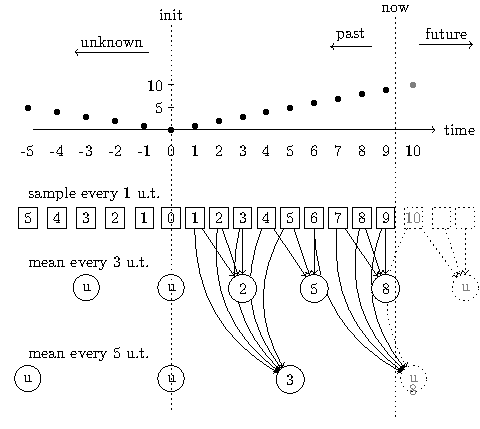
\includegraphics{fig_mtsms_sequence.pdf}
  \caption{Multiresolution snapshot diagram with regular sampling}
  \label{fig:mtsms:sequence}
\end{figure}


At the bottom of Figure~\ref{fig:mtsms:sequence} there is a diagram
showing the multiresolution action. The first row shows the numerical
time series' values corresponding to the above plot; the time series
is sampled every one unit of time. The second and the third row show a
particular schema of a multiresolution database consisting of two time
resolutions for the time series: one computes the mean of the sampled
values every three u.t.\ and the other computes the mean every five
u.t. In this example, computing the mean acts as selecting data
by aggregate statistics. All data stored before zero time are unknown
(\emph{u}) as has not been acquired. For the future values they are also
marked as \emph{u} until time advances.

The arrows of the figure show that every three sampled values a mean
is stored and, independently, every five values another mean is
stored. For the future values, dashed arrows show that if time
advances one u.t.\ then value 10 is sampled and the mean for time 10
can be computed resulting 8. However the mean every three values can not
be computed yet, so in this snapshot it keeps unknown value.





%%% Local Variables:
%%% TeX-master: "main"
%%% ispell-local-dictionary: "british"
%%% End:

%  LocalWords:  multiresolution TSMS MTSMS
